%% subsection prueba con usuarios finales
\subsection{Prueba con usuarios finales}
Para evaluar la usabilidad de la aplicación se utilizó el cuestionario SUS \footnote{SUS por sus siglas en ingles System Usability Scale permite medir que tan usable es un sistema mediante un cuestionario de 10 preguntas }, se trata de un cuestionario de 10 preguntas como se muestra en la Tabla \ref{tab:sus} con una escala de 5 puntos, donde 1 es muy en desacuerdo y 5 muy de acuerdo. 

En la Figura \ref{fig:sus} se muestra los resultados para la pregunta 1 del cuestionario SUS.

\begin{figure}[H]
    \centering
    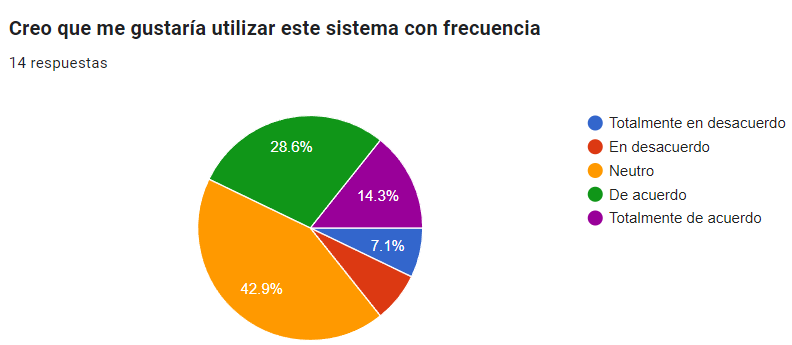
\includegraphics[width=0.8\textwidth]{../02Figures/03Chapter/sus.png}
    \caption{Resultados de la pregunta 1 del cuestionario SUS}\label{fig:sus}
\end{figure}

Las demas preguntas del cuestionario SUS se encuentran en el Anexo \ref{anexo:sus}.


%% Crea una tabla con las preguntas del cuestionario SUS

\begin{table}[H]
\centering
\label{tab:sus}
\begin{tabular}{|l|l|}
\hline
\textbf{Numero} & \textbf{Pregunta} \\ \hline
1 & Creo que me gustaría usar esta aplicación frecuentemente. \\ \hline
2 & Encontré la aplicación innecesariamente compleja. \\ \hline
3 & Creo que la aplicación es fácil de usar. \\ \hline
4 & Creo que necesitaría el apoyo de un experto para usar esta aplicación. \\ \hline
5 & Encontré que las diferentes funciones de la aplicación estaban bien integradas. \\ \hline
6 & Creo que la aplicación es muy inconsistente. \\ \hline
7 & Imagino que la mayoría de la gente aprendería a usar esta aplicación muy rápidamente. \\ \hline
8 & Encontré la aplicación muy difícil de usar. \\ \hline
9 & Me sentí muy confiado al usar la aplicación. \\ \hline
10 & Necesité aprender muchas cosas antes de poder empezar a usar la aplicación. \\ \hline
\end{tabular}
\caption{Cuestionario SUS}
\end{table}

El cuestionario fue aplicado a 14 usuarios, los resultados obtenidos se muestran en Anexo \ref{anexo:sus}. 
La puntuación obtenida fue de 70.89 puntos, lo que indica que la aplicación es usable. 